\documentclass[fullscreen=true, bookmarks=true, hyperref={pdfencoding=unicode}]{beamer}
\usepackage[utf8]{inputenc}                                % Кодировка
\usepackage[english,russian]{babel}                        % Переносы
\usepackage{xcolor}                                        % Работа с цветом
\usepackage{amsmath,amssymb,amsfonts}                      % Символы АМО
\usepackage{graphicx}                                      % Графика
\usepackage[labelsep=period]{caption}                      % Разделитель в подписях к рисункам и таблицам
\usepackage{hhline}                                        % Для верстки линий в таблицах
\usepackage{tikz}                                          % Для простых рисунков в документе
\usepackage{fancybox}                                      % Пакет для отрисовки рамок
\usepackage{verbatim}                                      % Для вставки кода в презентацию
\usepackage{animate}                                       % Для вставки видео в презентацию
\usepackage{xmpmulti}                                      % Для вставки gif в презентацию
\usepackage{multirow}

\usetikzlibrary{arrows,snakes,backgrounds}                 % Для отрисовки стрелок

\graphicspath{{images/}}                                   % Путь до рисунков
\setbeamertemplate{caption}[numbered]                      % Включение нумерации рисунков

\definecolor{links}{HTML}{2A1B81}                          % blue for url links
\hypersetup{colorlinks,linkcolor=,urlcolor=links}          % nothing for others

\usetheme{boxes}
\usecolortheme{crane}

\usepackage{pmostowsky_commands}

\newtheorem*{question}{Вопрос}

\title{Лекция 8. Гауссовские процессы.\\ Байесовская оптимизация}
\author{Петр Мостовский}
\institute{МКН СПбГУ}
\date{7 апреля 2022}
\titlegraphic{
\includegraphics[keepaspectratio,width=0.5\textwidth]{logo_fmkn.png}}


\begin{document}

\begin{frame}
    \transdissolve[duration=0.2]
    \titlepage
\end{frame}


\begin{frame}{}

    \centerline{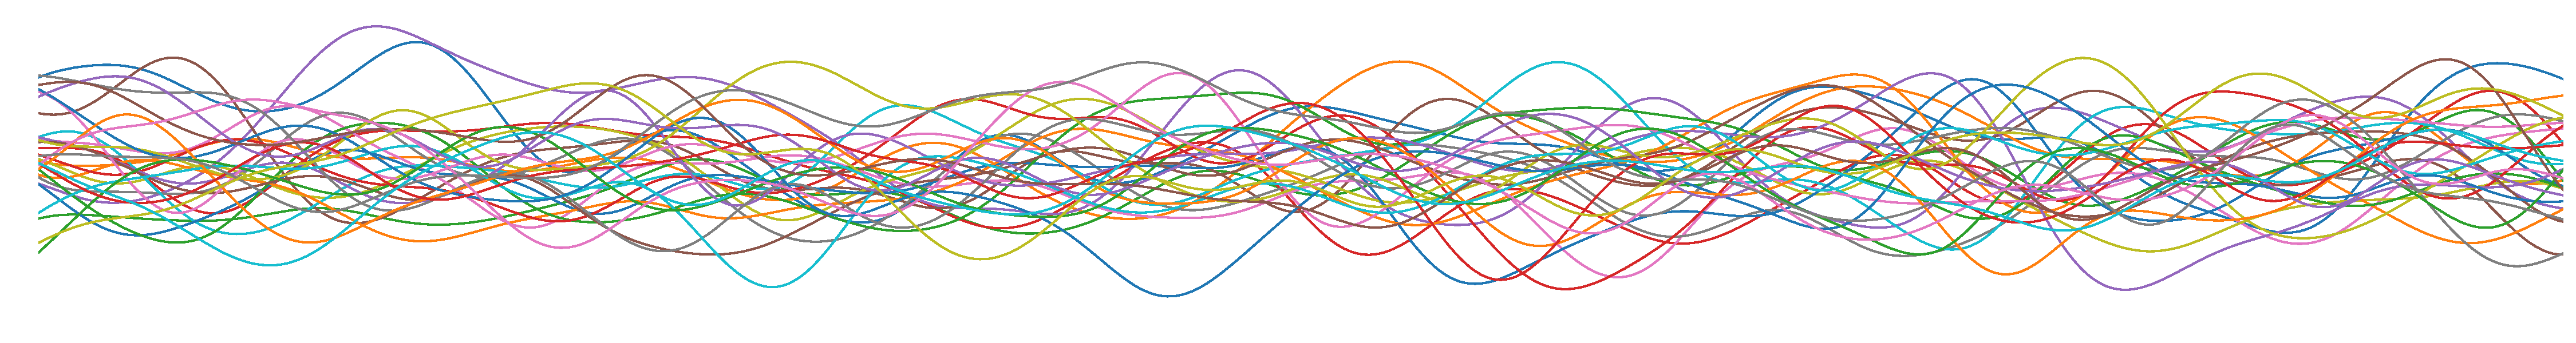
\includegraphics[]{logo-samples.pdf}}

\end{frame}


%%% Байесовская оптимзиция
\begin{frame}{Черный ящик}

\begin{itemize}
    \item<1-> Черный ящик $f(x)$ --- сложновычислимая функция. Градиенты $f$, как правило, недоступны
    \item<2-> Хотим найти
    \[
        x_{*} = \argmax_{x \in \c{X}} f(x)
    \]
    \item<3-> Некоторые стратегии
        \begin{itemize}
            \item<4-> Grid search. Перестает работать с ростом размерности $\c{X}$
            \item<5-> Random search. Никак не  использует доступную информацию об $f$
            \item<6-> Численные градиенты. Вычисление градиента так же дорого, как вычисление самой $f$. Использует только последние несколько значений $f$
        \end{itemize}
\end{itemize}

\end{frame}

\begin{frame}{Примеры черных ящиков}

\begin{itemize}
    \item<1-> Качество обученной нейросети на валидационном датасете
    \only<2->{(параметры: learning rate, momentum, batch size и т.д.)}
    \item<3-> Дизайн экспериментов
    \item<4-> Дизайн машин (например, крыла самолета)
    \item<5-> et cetera...
\end{itemize}

\end{frame}


\begin{frame}{Предположения о черном ящике}
    \begin{itemize}
        \item<1-> $f$ сложновычислима
        \item<2-> $f$ непрерывная, но у нее нет особой структуры (например, выпуклости)
        \item<3-> $\c{X}$ компактно
        \item<3-> градиенты $f$ недоступны
        \item<4-> значения $f$ могут быть шумными
    \end{itemize}
\end{frame}

\begin{frame}{Байесовская оптимизация}
    \begin{itemize}
        \item<1-> Поскольку $f$ --- черный ящик, будем воспринимать $f$ как случайную (введем prior $p(f)$)
        \item<2-> Будем обновлять prior с помощью теоремы Байеса, учитывая наблюдаемые значения $f(x_1), f(x_2), \ldots$
        \item<3-> Будем искать нужный нам аргмаксимум $x_*$ исходя из posterior
        $$ p(f(x_*) | f(x_1), f(x_2), \ldots) $$
    \end{itemize}
\end{frame}

% \begin{frame}{Frame Title}

% \end{frame}


\begin{frame}{Иллюстративный пример}
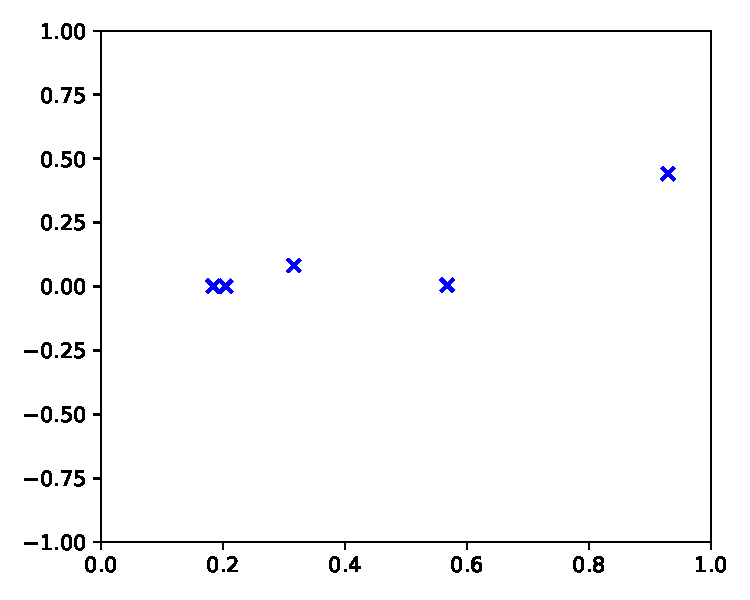
\includegraphics[width=\textwidth]{01_bayesopt_data.pdf}
\end{frame}

\begin{frame}{Гауссовские процессы}

    \begin{itemize}
        \item<1-> Нам нужно ввести какое-то априорное распределение на $f$
        \item<2-> Какой подходящий prior выбрать? \only<3->{Гауссовский процесс!}
        \item<4-> Используем информацию о всех имеющихся значениях $f$
        \item<5-> Используем апостериорное распределение, чтобы выбрать кандидата на максимум
    \end{itemize}

\end{frame}

\begin{frame}{Иллюстративный пример}
    \only<1>{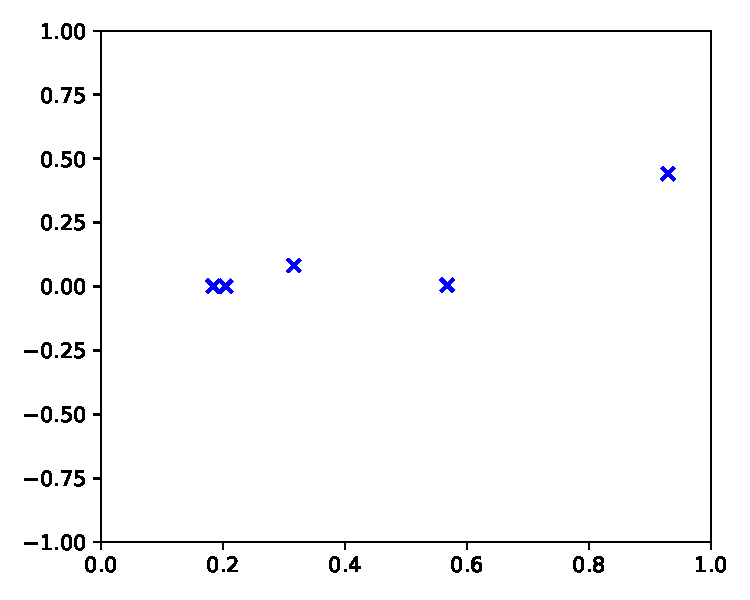
\includegraphics[width=\textwidth]{01_bayesopt_data.pdf}}
    \only<2>{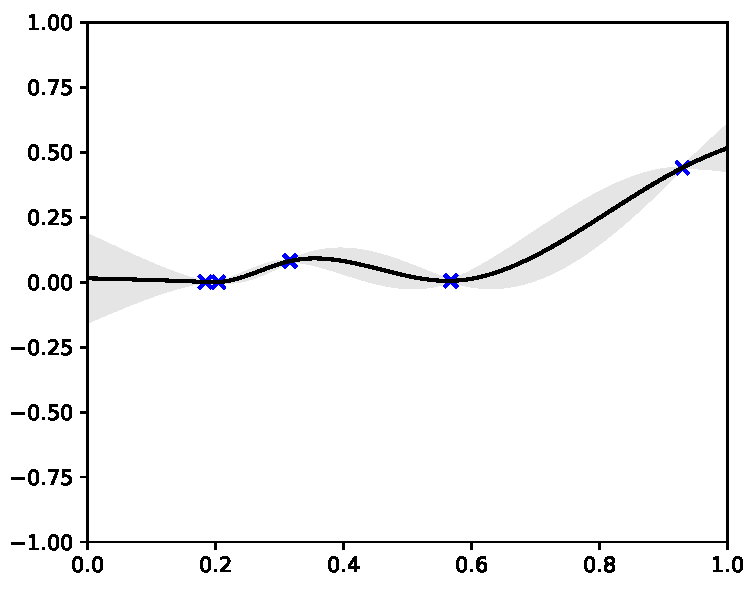
\includegraphics[width=\textwidth]{02_bayesopt_gp_0.pdf}}
\end{frame}

\begin{frame}{Acquisition function}

    \begin{itemize}
        \item<1-> Как выбрать кандидата на максимум?
        \item<2-> У нас есть целое апостериорное распределение, давайте используем его
        \item<3-> Например, выберем $x_*$ такой, что
        \[
            x_* = \argmax_{x \in \c{X}} P(f(x) \geq f^{+} + \varepsilon),
        \]
        где $f^{+}$ -- текущее наилучшее значение
        \item<4-> Функция
        \[
            \alpha(x; f^{+}) := P(h(x) \geq f^{+} + \varepsilon)
        \]
        называется Probability of Improvement
        \item<5-> Для GP prior, Probability of Improvement считается аналитически
    \end{itemize}

\end{frame}

\begin{frame}{Иллюстративный пример}
    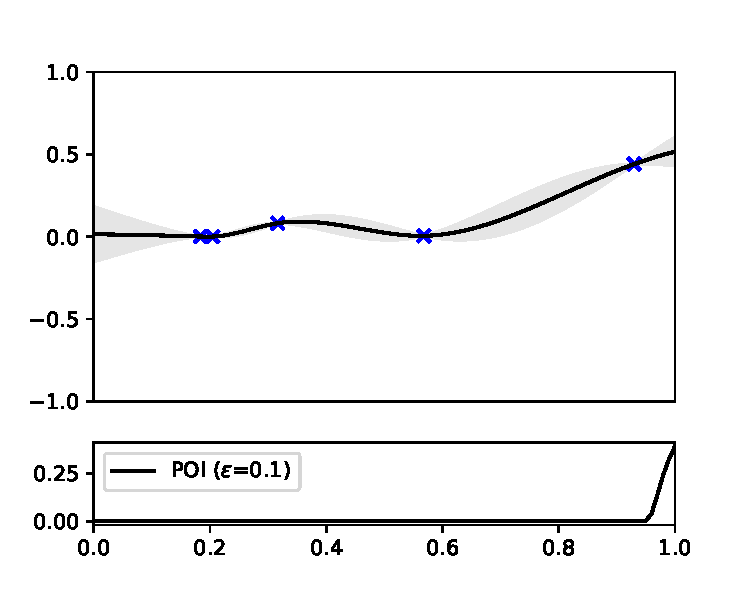
\includegraphics[width=\textwidth]{03_bayesopt_gp_0_poi.pdf}
\end{frame}

\begin{frame}{Acquisition function}

\begin{itemize}
    \item<1-> Более общо, вводится acqusition function $\alpha(x)$, которая
    \begin{itemize}
        \item<2-> просто вычислима
        \item<3-> отражает наши представления о том, где находится кандидат на максимум, исходя из апостериорного распределения
    \end{itemize}
    \item<4-> Примеры acquisition function \onslide<5->{:}
    \begin{itemize}
        \item<5-> Expected Improvement
        \[
            \alpha_{EI}(x) = \bbE( \max(0, h(x) - f^{+}) | \c{D} )
        \]
        \item<6-> Upper Confidence Bound
        \[
            \alpha_{UCB}(x) = \mu(x) + \lambda \sigma(x)
        \]
        \item<7-> И другие...
    \end{itemize}
\end{itemize}

\end{frame}

\begin{frame}{Иллюстративный пример}
     \only<1>{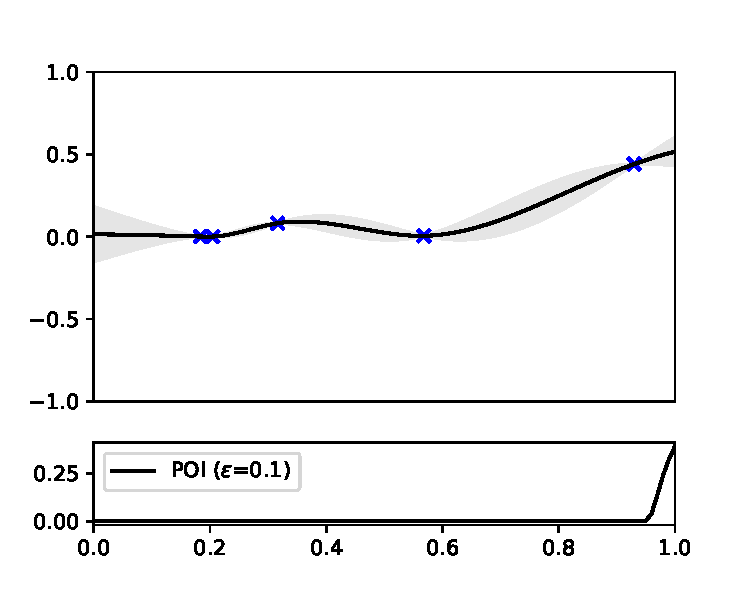
\includegraphics[width=\textwidth]{03_bayesopt_gp_0_poi.pdf}}
     \only<2>{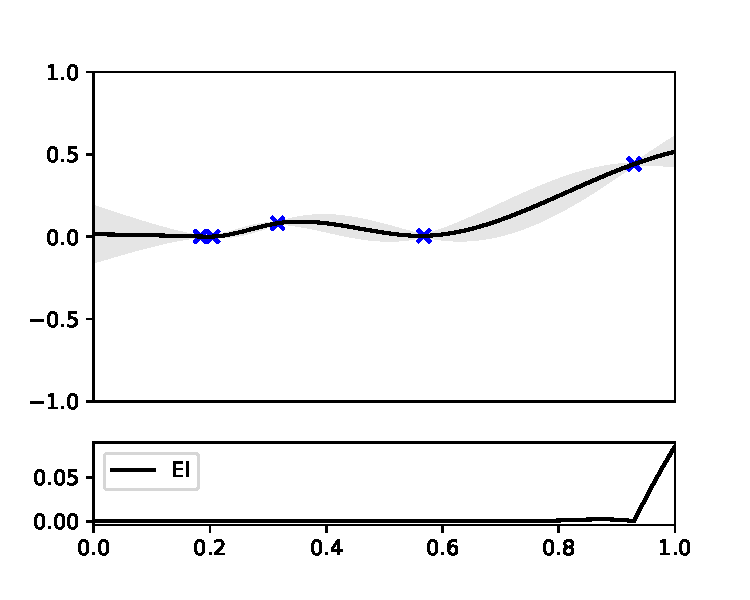
\includegraphics[width=\textwidth]{03_bayesopt_gp_0_ei.pdf}}
     \only<3>{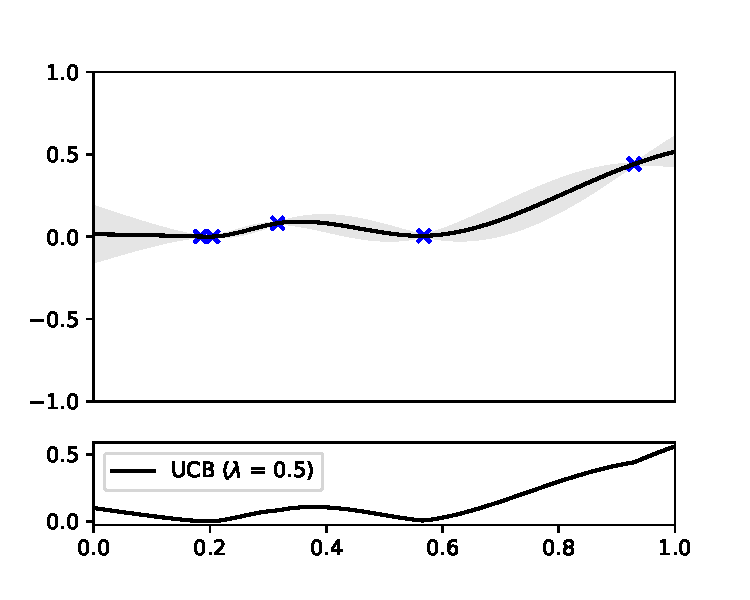
\includegraphics[width=\textwidth]{03_bayesopt_gp_0_ucb.pdf}}
\end{frame}

\begin{frame}{Формулы}

    Probability of Improvement
    \<
        \onslide<1-5>{\alpha_{POI}(x; f^{+}) := P(h(x) \geq f^{+} + \varepsilon) = } \only<2-5>{\\
        P(\mu(x) + \sigma(x) u \geq f^{+} + \varepsilon) = }
        \onslide<3-5>{\\
        P(u \geq \frac{f^{+} + \varepsilon - \mu(x)}{\sigma(x)}) = }
        \onslide<4-5>{
        \\
        1 - P\Bigg(u \leq \frac{f^{+} + \varepsilon - \mu(x)}{\sigma(x)}\Bigg) =}
        \onslide<5>{\\
        \Phi\Bigg(-\frac{f^{+} + \varepsilon - \mu(x)}{\sigma(x)}\Bigg)}
    \>
\end{frame}

\begin{frame}{Формулы}
    Expected Improvement
    \<
        \onslide<1->{\alpha_{EI}(x) = \bbE( \max(0, h(x) - f^{+} ) =}
        \onslide<2->{\\
        \int_{-\infty}^{\infty} \max(0, \mu(x) + \sigma(x)u - f^{+}) \phi(u) du = }
        \onslide<3->{\\ \Bigg[ z := \frac{f^+ - \mu(x)}{\sigma(x)} \Bigg]  }
        \\
        \onslide<4->{ \int_{z}^{\infty} (\mu(x) - f^+ + \sigma(x) u) \phi(u) du = }
        \onslide<5->{\\ (\mu(x) - f^+) \Phi(-z) + \sigma(x) \int_{z}^{\infty} u \phi(u) du = }
        \onslide<6->{\\ (\mu(x) - f^+) \Phi(-z) + \sigma(x) \phi(z) }
    \>
\end{frame}

\begin{frame}{Exploration vs Exploitation}
    Два режима оптимизации:
    \begin{itemize}
        \item<1-> Exploration. ``Исследование'' областей с высокой неопределенностью.
        \item<2-> Exploitation. ``Использование'' знаний об области с правдоподобным максимумом.
        \item<3-> Exploration/exploitation tradeoff --- хотим исследовать области с высокой неопределенностью, но не хотим тратить слишком много ресурсов
        \item<4-> В UCB за tradeoff отвечает $\lambda$
        \[
            \alpha_{UCB}(x) = \mu(x) + \lambda \sigma(x)
        \]
    \end{itemize}
\end{frame}

\begin{frame}{Стратегия поиска максимума}
    \begin{enumerate}
        \item<1-> Warmup. Получим ``начальные'' значения $f(x_1), \ldots, f(x_n)$. Датасет $\c{D}_n := (x_i, y_i)$
        \item<2-> Обучим гауссовский процесс на данных $\c{D}_n$
        \item<3-> Найдем кандидата на максимум $x_{n+1} := \argmax_{x \in \c{X}} \alpha(x)$
        \item<4-> Вычислим значение $y_{n+1}$ в $x_{n+1}$
        \item<5-> Добавим $(x_{n+1}, y_{n+1})$ в датасет $\c{D}_{n+1}$
        \item<6-> Вернемся к пункту 2.
        \item<7-> ???
        \item<8> PROFIT!
    \end{enumerate}
\end{frame}

\begin{frame}{Иллюстративный пример}
    \only<1>{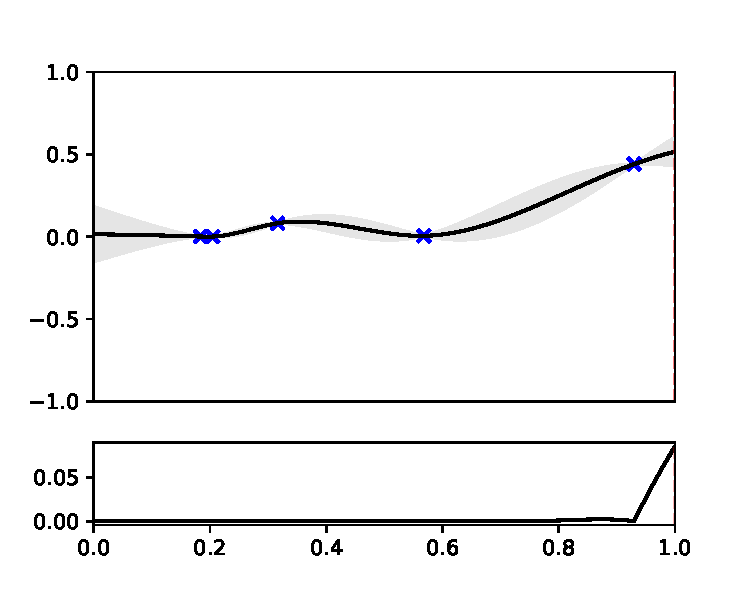
\includegraphics[width=\textwidth]{04_bayesopt_gp_0_ei.pdf}}
    \only<2>{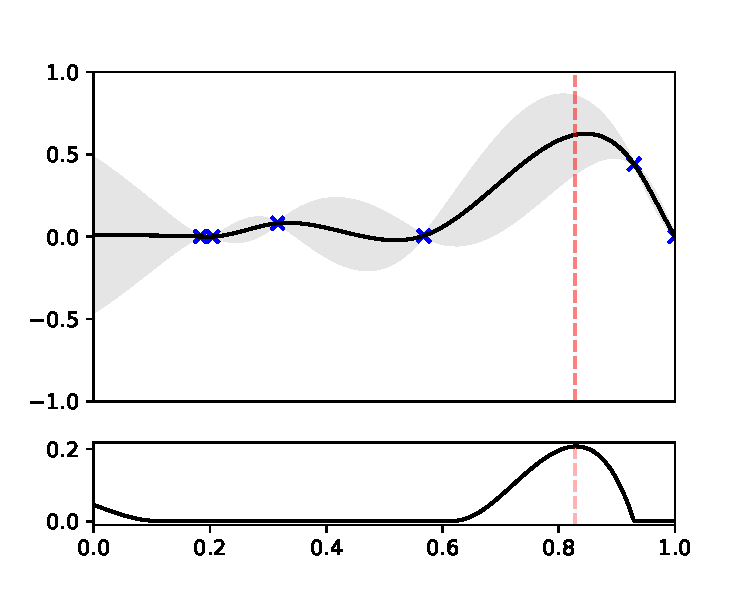
\includegraphics[width=\textwidth]{04_bayesopt_gp_1_ei.pdf}}
    \only<3>{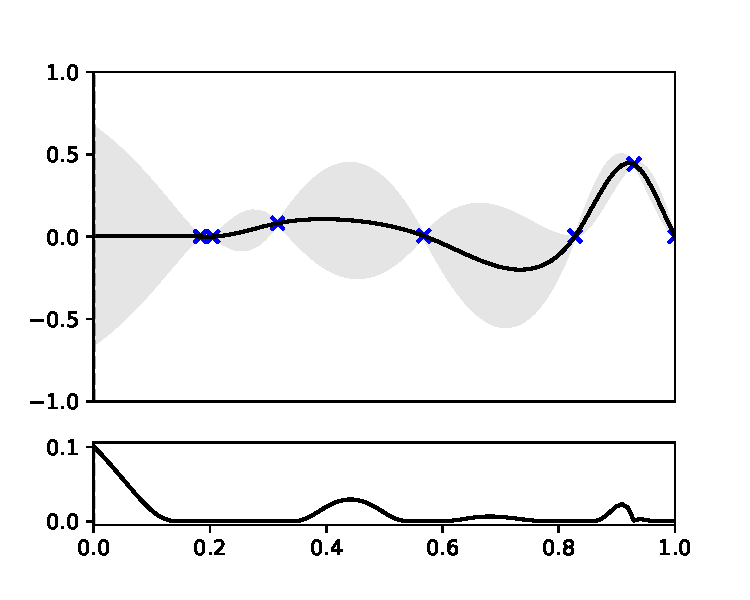
\includegraphics[width=\textwidth]{04_bayesopt_gp_2_ei.pdf}}
    \only<4>{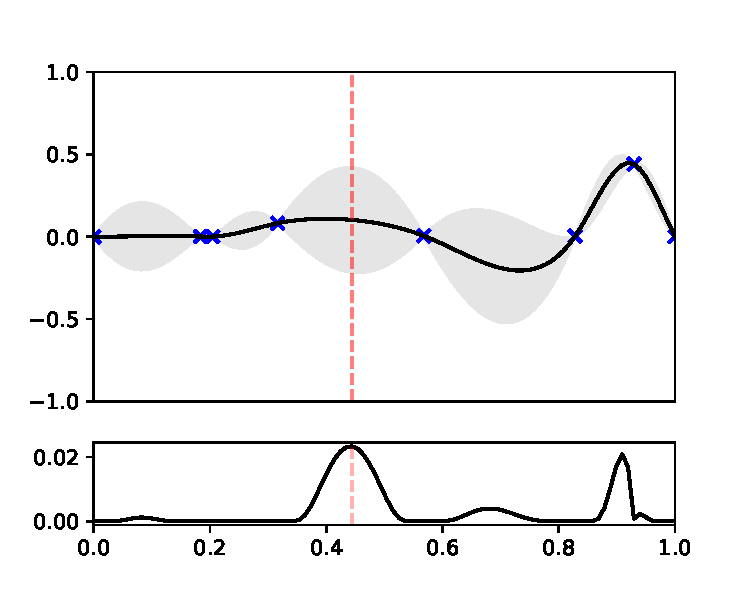
\includegraphics[width=\textwidth]{04_bayesopt_gp_3_ei.pdf}}
    \only<5>{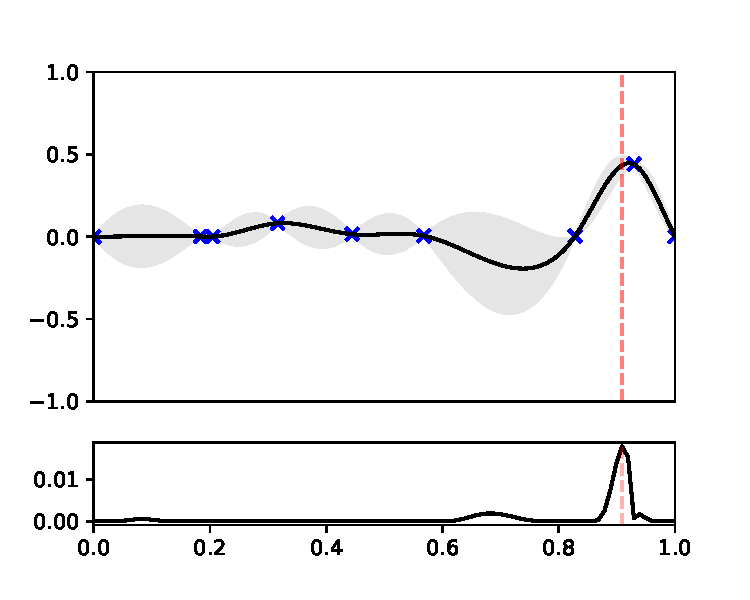
\includegraphics[width=\textwidth]{04_bayesopt_gp_4_ei.pdf}}
    \only<6>{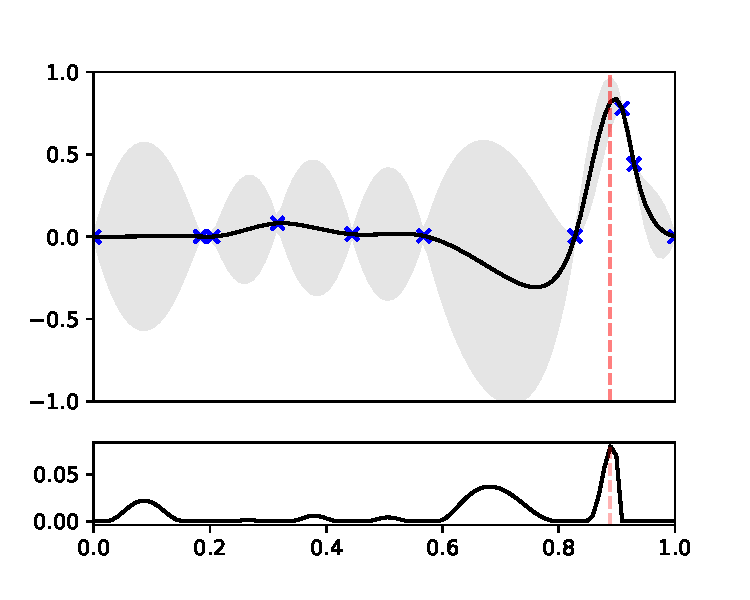
\includegraphics[width=\textwidth]{04_bayesopt_gp_5_ei.pdf}}
    \only<7>{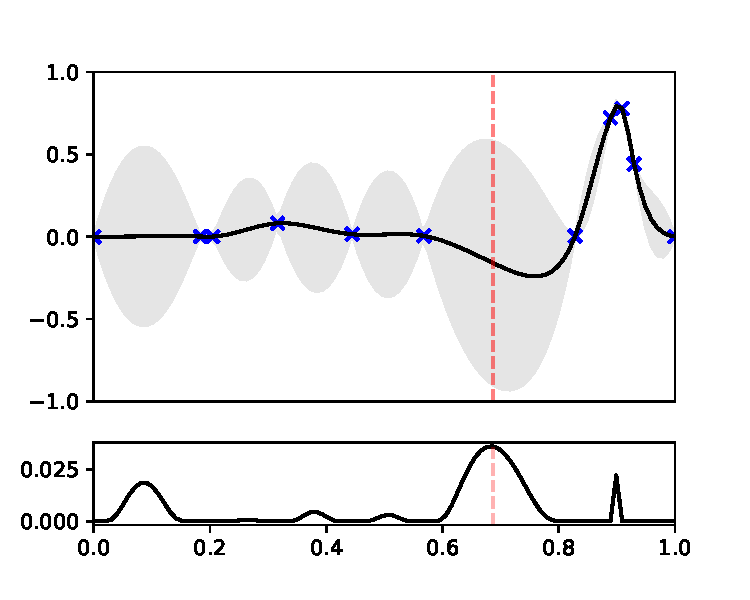
\includegraphics[width=\textwidth]{04_bayesopt_gp_6_ei.pdf}}
    \only<8>{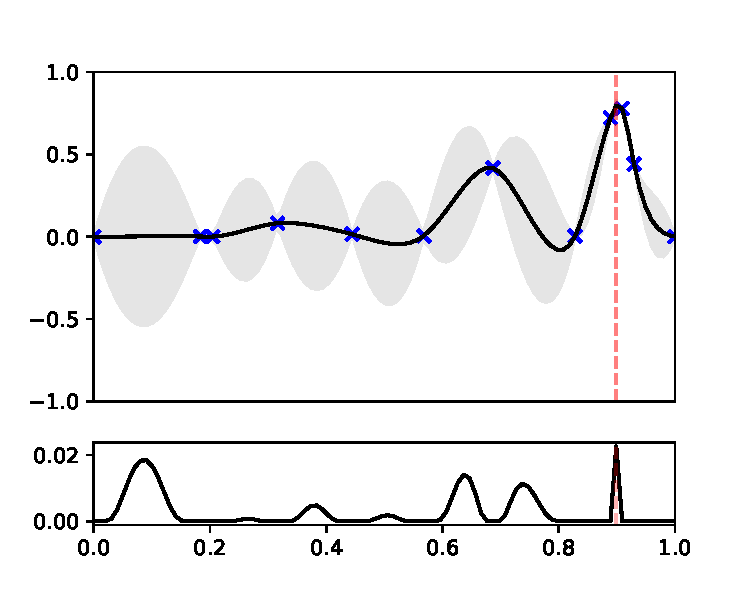
\includegraphics[width=\textwidth]{04_bayesopt_gp_7_ei.pdf}}
    \only<9>{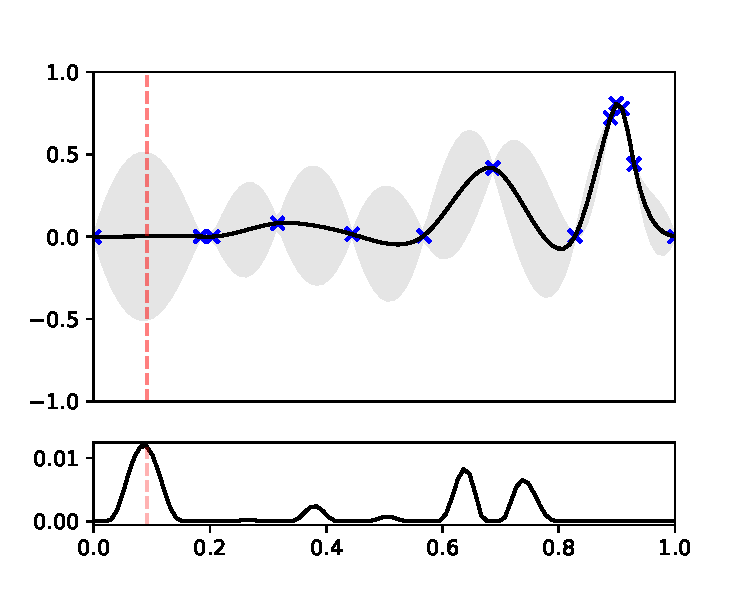
\includegraphics[width=\textwidth]{04_bayesopt_gp_8_ei.pdf}}
    \only<10>{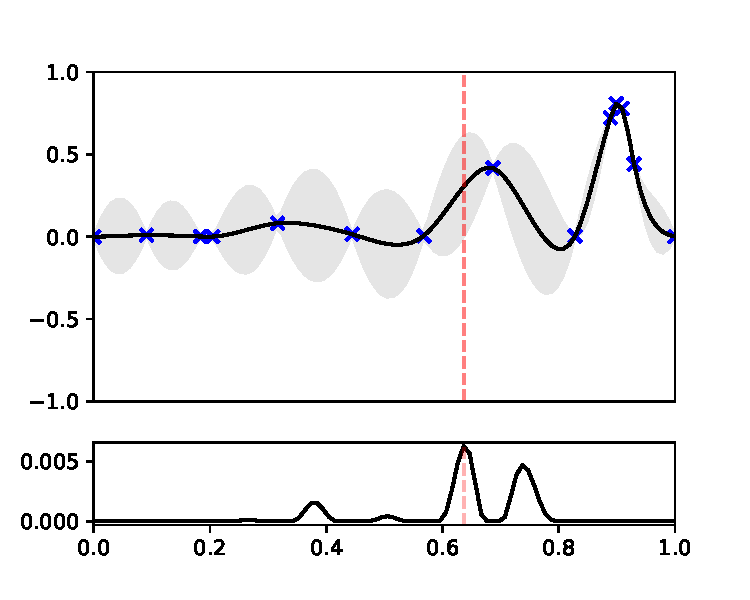
\includegraphics[width=\textwidth]{04_bayesopt_gp_9_ei.pdf}}
    \only<11>{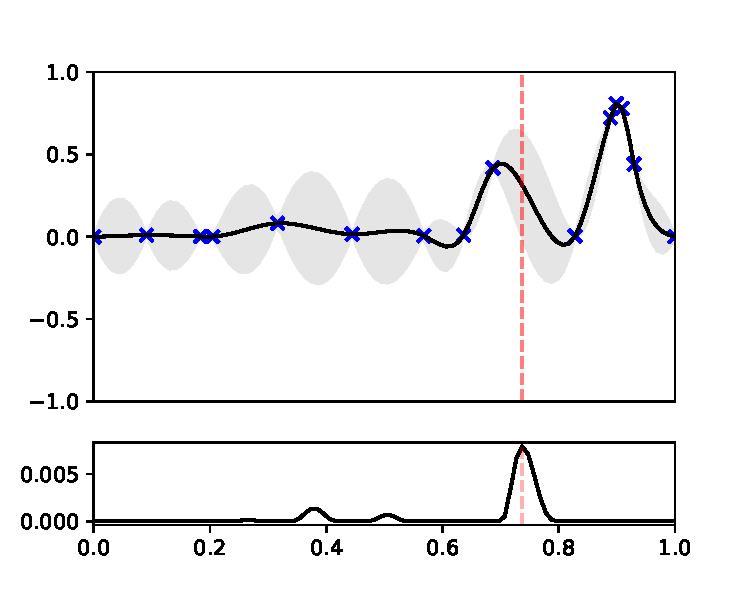
\includegraphics[width=\textwidth]{04_bayesopt_gp_10_ei.pdf}}
    \only<12>{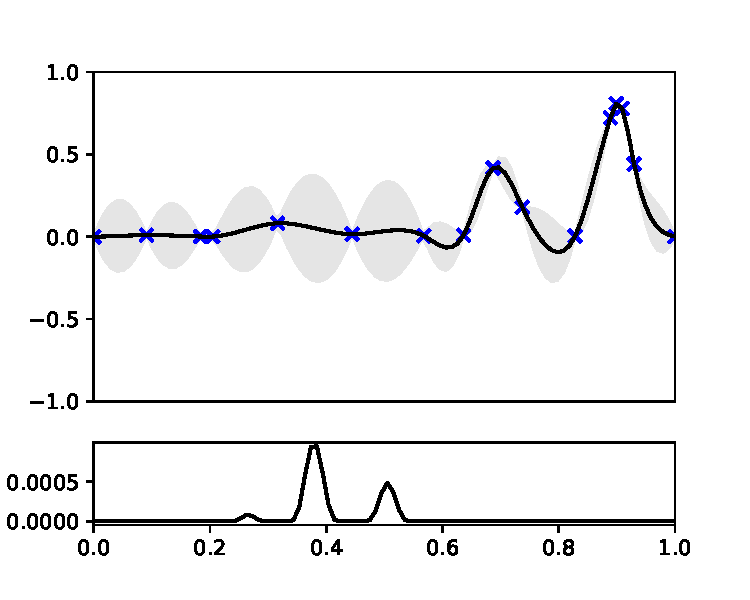
\includegraphics[width=\textwidth]{04_bayesopt_gp_11_ei.pdf}}
    \only<13>{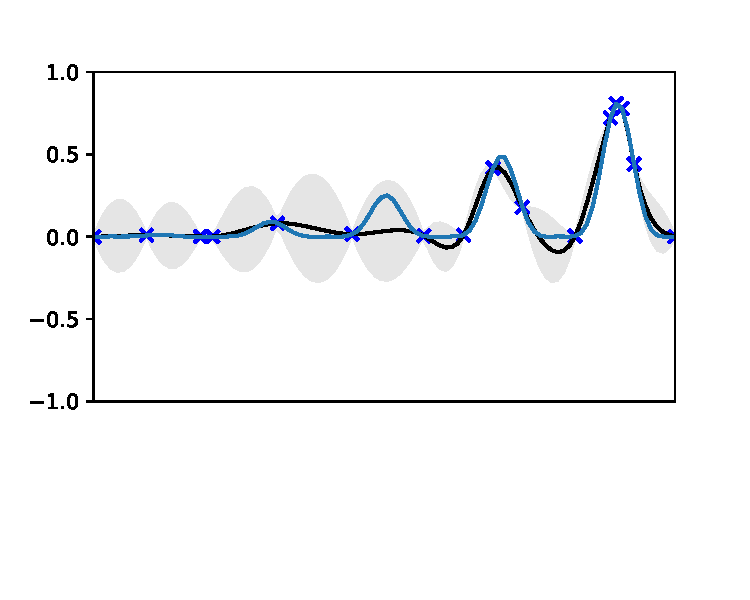
\includegraphics[width=\textwidth]{04_bayesopt_truth.pdf}}
\end{frame}

\begin{frame}{Thomspon Sampling}

    \begin{itemize}
        \item<1-> $f$ случайна, и ее максимум -- случайная величина
        \<
            x_{*} =& \argmax_{x \in \c{X}} f(x) \\
            p(x_* | \c{D}) =& \text{?}
        \>
        где $\c{D} = (x_i, y_i)_{i=1}^{n}$ --- наблюдаемые данные
        \item<2->
        \[
            p(x_* | \c{D}) = \int p(x_* | g, \c{D}) p(g | \c{D}) dg
        \]
        где $g$ -- гауссовский процесс, $p(x_* | g)$ --- масса на аргмаксимуме траектории $g | \c{D}$.
        \item<3-> Thompson sampling\onslide<4->{:}
        \begin{itemize}
            \item<4-> Сэмплируем траекторию $g | \c{D}$ \onslide<5->{(формула Матерона)}
            \item<6-> Находим ее аргмаксимум
        \end{itemize}
    \end{itemize}

\end{frame}

\begin{frame}{Иллюстративный пример}
    \only<1>{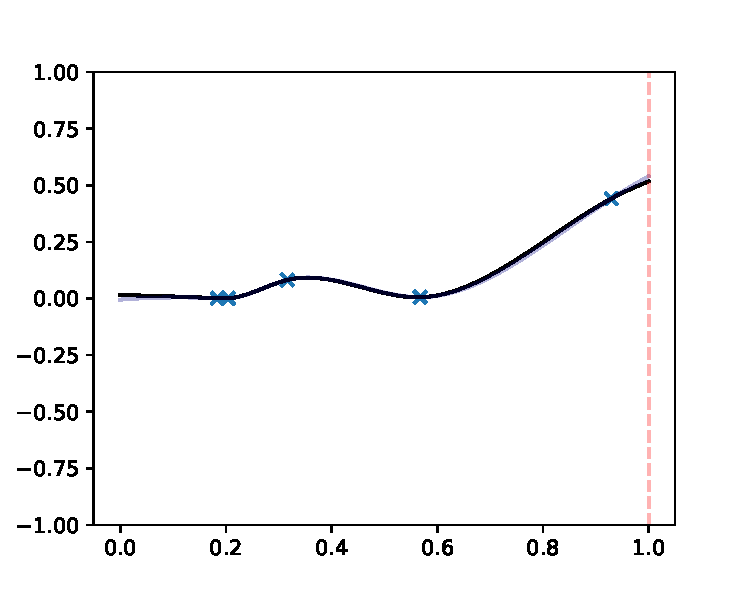
\includegraphics[width=\textwidth]{05_bayesopt_gp_0_TS.pdf}}
    \only<2>{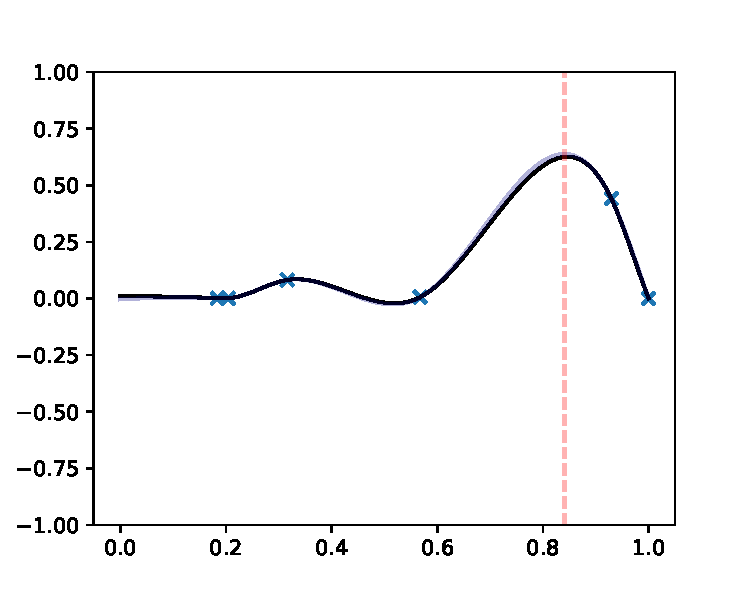
\includegraphics[width=\textwidth]{05_bayesopt_gp_1_TS.pdf}}
    \only<3>{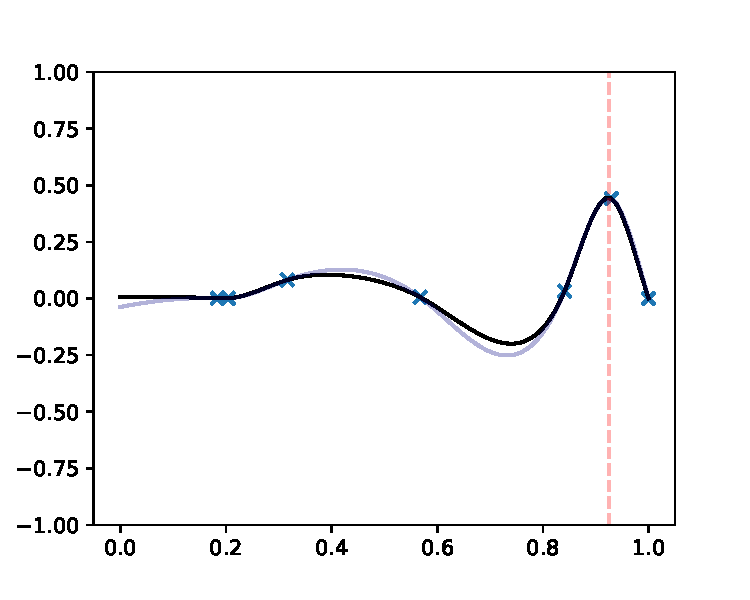
\includegraphics[width=\textwidth]{05_bayesopt_gp_2_TS.pdf}}
    \only<4>{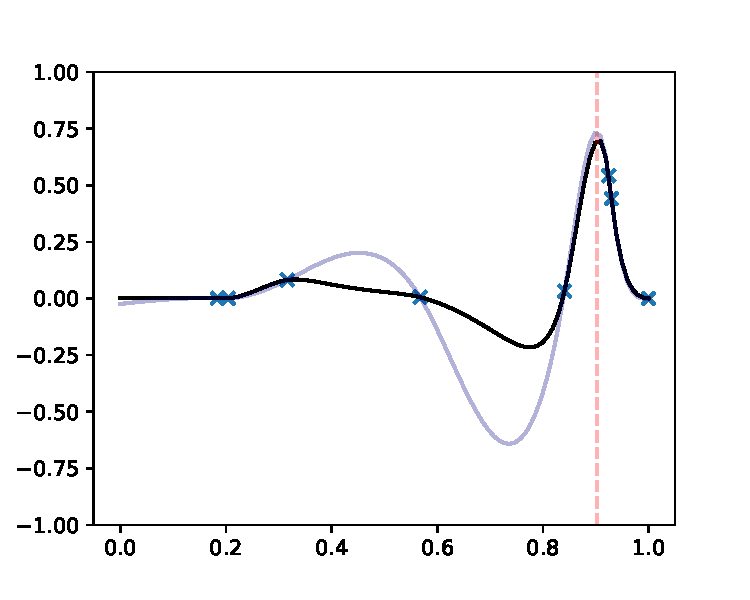
\includegraphics[width=\textwidth]{05_bayesopt_gp_3_TS.pdf}}
    \only<5>{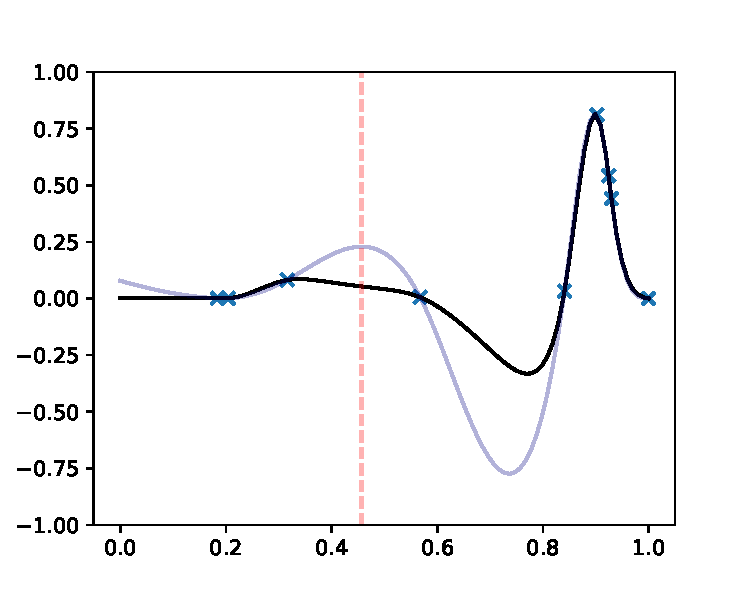
\includegraphics[width=\textwidth]{05_bayesopt_gp_4_TS.pdf}}
    \only<6>{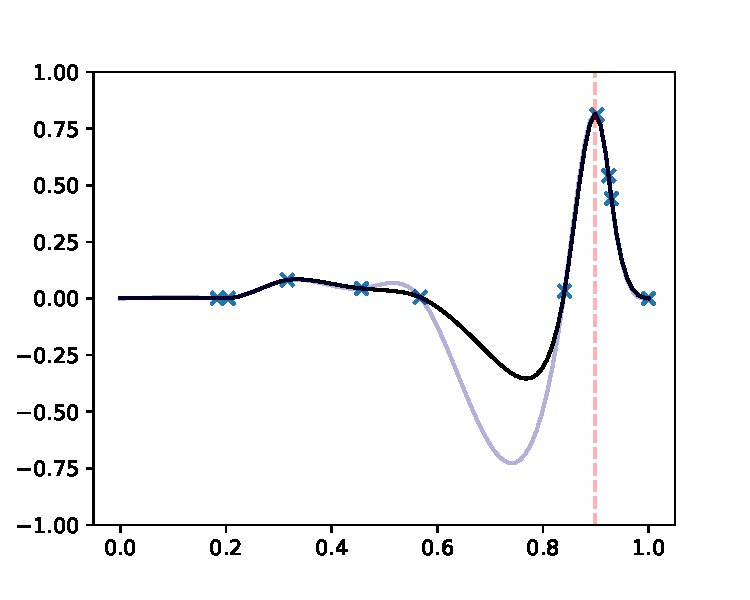
\includegraphics[width=\textwidth]{05_bayesopt_gp_5_TS.pdf}}
    \only<7>{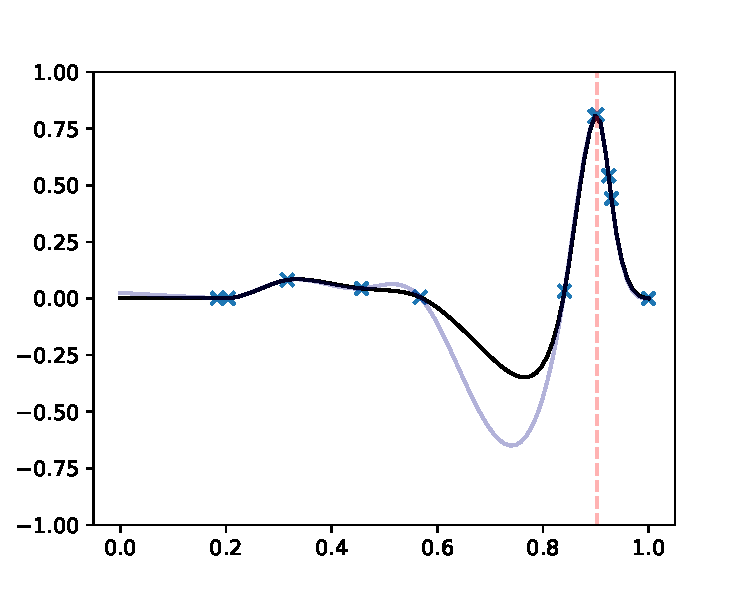
\includegraphics[width=\textwidth]{05_bayesopt_gp_6_TS.pdf}}
\end{frame}

\begin{frame}{Regrets}

\begin{itemize}
    \item Regret
    \[
    r_n := f(x_*) - f(x_n)
    \]
    \item Cumulative regret
    \[
    R_n := \sum_{i=1}^{n} [ f(x_*) - f(x_i) ]
    \]
    \item No regret:
    \[
        \frac{R_n}{n} \longrightarrow 0
    \]
\end{itemize}

\end{frame}

\begin{frame}{No Silver Bullet}

\onslide<1->{
\begin{exampleblock}{Выбор ядра для априорного гауссовского процесса}
Нужно каким-то образом выбирать ядро для ГП --- это вводит новые гиперпараметры, которые мы должны найти, оптимизируя MLL.
\end{exampleblock}
}

\onslide<2->{
\begin{exampleblock}{Внутренняя оптимизация}
Оптимизируем acquistion function, чтобы найти кандидата на минимум --- нет гарантий сходимости к глобальному максимуму.
\end{exampleblock}
}

\onslide<3->{
\begin{exampleblock}{Проблема Large dimensions}
Высокая размерность пространства поиска плохо дружит с байесовской оптимизацией.
Rule of thumb --- 20D.
\end{exampleblock}
}

\end{frame}

\begin{frame}{}

\end{frame}

\begin{frame}{ARD}

    \begin{itemize}
        \item<1-> Стационарное ядро
        \[
        k(x, x^\prime) = k(\Vert x - x^\prime \Vert) = k\left(\sqrt{\sum_{d=1}^{D} (x_d - x^\prime_d)^2} \right)
        \]
        \item<2-> Параметр масштаба (lengthscale)
        \[
            \frac{\sqrt{\sum_{d=1}^{D} (x_d - x^\prime_d)^2}}{\ell}
        \]
        \item<3-> Automatic Relevance Determination
        \[
            \sqrt{\sum_{d=1}^{D} \left( \frac{x_d - x^\prime_d}{\ell_{d}} \right)^2 }
        \]
    \end{itemize}

\end{frame}

\begin{frame}{}
    \centerline{Спасибо!}
\end{frame}


\end{document}
